
\chapter{Solid mechanics}
	\section{Continuum mechanics}
		\subsection{Statics}
		
		\begin{wrapfigure}[8]{l}{5cm}
		\vspace{-5mm}	
		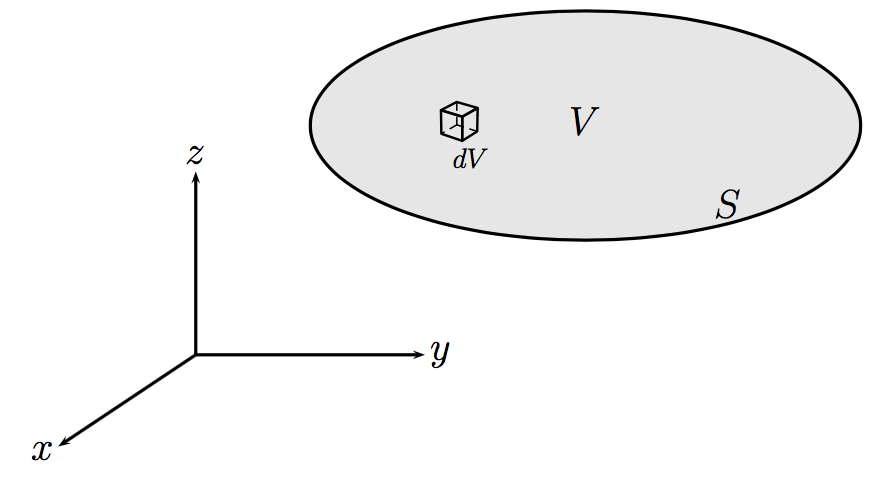
\includegraphics[scale=0.3]{ch3/1}
		\captionof{figure}{}
		\end{wrapfigure}		
		We will establish the governing equations in \textbf{continuum} mechanics. Consider a volume V delimited by a surface S, defined in a right-handed Cartesian coordinate. Continuum means, despite the microscopic description, that the material is assumed to behave as a continuum whole body. We can define the physical quantity in every point (x,y,z) of V by means of continuous function:
		
		\begin{equation}
		\rho = \lim _{dV\rightarrow 0} \frac{dm}{dV}.
		\end{equation}
		
		In addition, we assume the \textbf{differentiability} that allows to write these equations in function of infinitesimal quantities. We also assume that the material is \textbf{homogeneous} and \textbf{isotropic} (same mechanical properties in all directions). Birth and propagation of cracks are causes of loss of continuity. In this case the continuity approach is not valid anymore. In numerical methods, it requires extensions as X-FEM and others. \\
		
		There are two types of external forces: 
		\begin{itemize}
			\item[•] \textbf{Body forces b:} acting throughout the volume $V$. This depending on position, the resultant:
			
			\begin{equation}
				\mathbf{f}^v = \int _V \mathbf{b}(x,y,z) \rho (x,y,z)\, dV.
			\end{equation}
			
			In statics, gravity loads are the main body forces: 
			
			\begin{equation}
			\mathbf{b} = \left[
			\begin{array}{c}
			0\\
			0\\
			- g
			\end{array}
			 \right],
			\end{equation}
			z assumed to be the vertical axis oriented upwards. 
			
		\	\item[•] \textbf{Contact forces t:} present at the contact between two points or surfaces. In practice it is either external forces on S or reactions at attachment points. 
		\end{itemize}
		
		\begin{wrapfigure}[8]{l}{5cm}
		\vspace{-5mm}	
		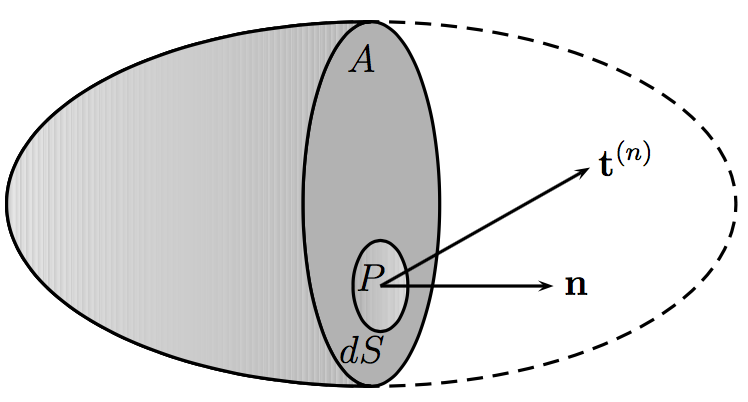
\includegraphics[scale=0.3]{ch3/2}
		\captionof{figure}{}
		\end{wrapfigure}		
		To introduce the notion of \textbf{Cauchy stresses}, let's cut a section $A$ in the a volume $V$. The arbitrary surface $dS$ on $A$ is characterized by a resultant force $d\mathbf{f}$ and a resultant moment $d\mathbf{m}$. The \textbf{Cauchy stress vector} is defined as: 
		
		\begin{equation}
		\mathbf{t}^{(n)} = \lim _{dS\rightarrow 0} \frac{d\mathbf{f}}{dS}. 
		\end{equation}
		
		For the rest of the course we will assume $d\mathbf{m}/dS = 0$. Remark that $\mathbf{t}^{(n)}$ is associated to a certain normal, if we make another cut $A'$, we will have another normal $\bm{n}'$ and a different stress vector. We only have that $\mathbf{t}^{(n)} = -\mathbf{t}^{(-n)}$ (action-reaction). \\
		
		\begin{wrapfigure}[8]{r}{8.5cm}
		\vspace{-5mm}	
		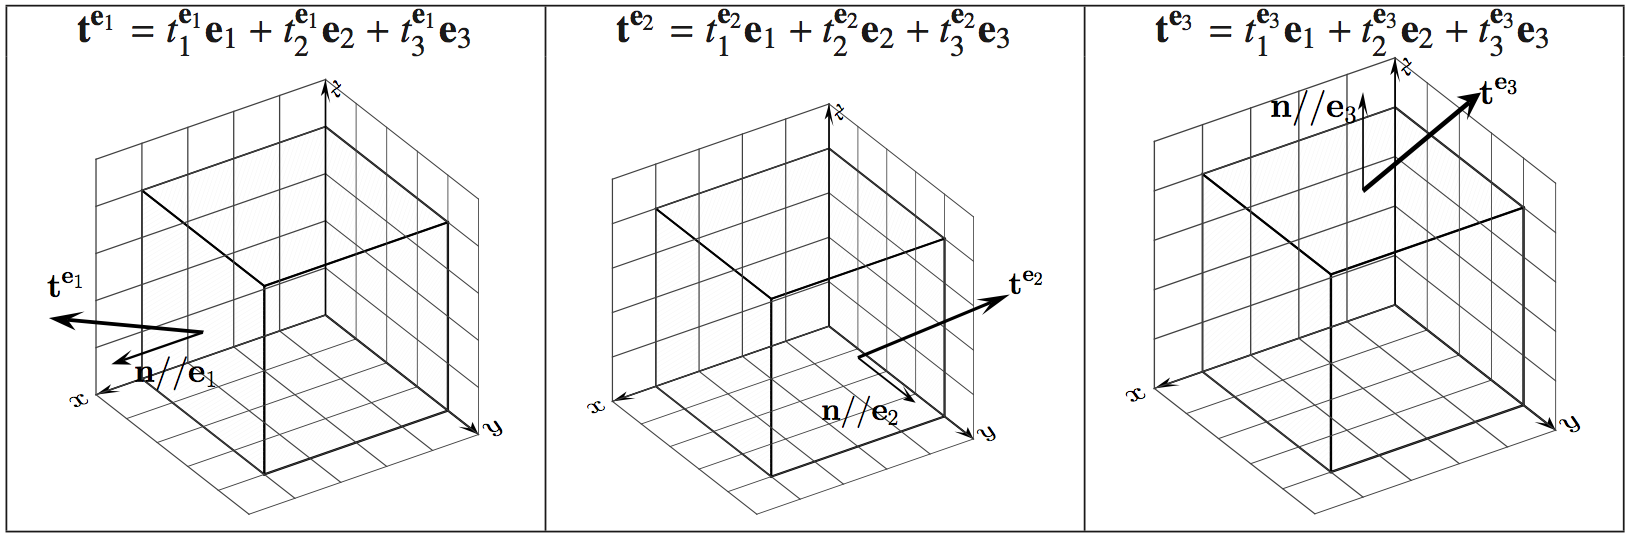
\includegraphics[scale=0.3]{ch3/3}
		\captionof{figure}{}
		\label{fig:3.3}
		\end{wrapfigure}		
		Since each direction is associated to a stress vector, we define the second-order \textbf{stress tensor} $\bm{\bar{\bar{\tau}}}$. For this, we make the stress vectors defines for the three coordinate planes related to the unit normals $\bm{e}^{(1)}, \bm{e}^{(2)}, \bm{e}^{(3)}$ (see \autoref{fig:3.3}). From this tensor, we can find any stress vector by projecting the tensor on the normal $\bm{n}$ associated to the cutting plane:
		
		\begin{equation}
			\bm{\bar{\bar{\tau}}. n} = 
			\left[
			\begin{array}{ccc}
			\tau _{xx} & \tau _{xy} & \tau _{xz}\\
			\tau _{yx} & \tau _{yy} & \tau _{yz}\\
			\tau _{zx} & \tau _{zy} & \tau _{zz}
			\end{array}
			\right]
			\left[
			\begin{array}{c}
			n_1\\
			n_2\\
			n_3
			\end{array}
			\right].
		\end{equation}
		
		As reminder of the notation, $\bm{\tau} _{xx} = \bm{\sigma} _x$ (normal stress, $0<\rightarrow$ tension, $<0 \rightarrow$ compression) points the normal component in x direction, xy (shear stress) will points to the vector of the plane $\perp x$ oriented to y and xz is the same but oriented to z. Stresses are measured in $N/m^2 =$ Pa.\\
		
		We have to make the difference between 0-order, 1-order and 2-order tensors. The first means that the same scalar value is associated to each direction of the 3D space (does not depend on the orientation). For a 1-order tensor $\bm{v}$, assuming a given orientation $\bm{d}$, a scalar value is associated to $\bm{d}$ by $v_d = \bm{d}.\bm{v}$. This scalar change in function of the considered direction. And for the last, we have a different vector for any direction. \\
		
		\begin{wrapfigure}[8]{l}{7cm}
		\vspace{-10mm}	
		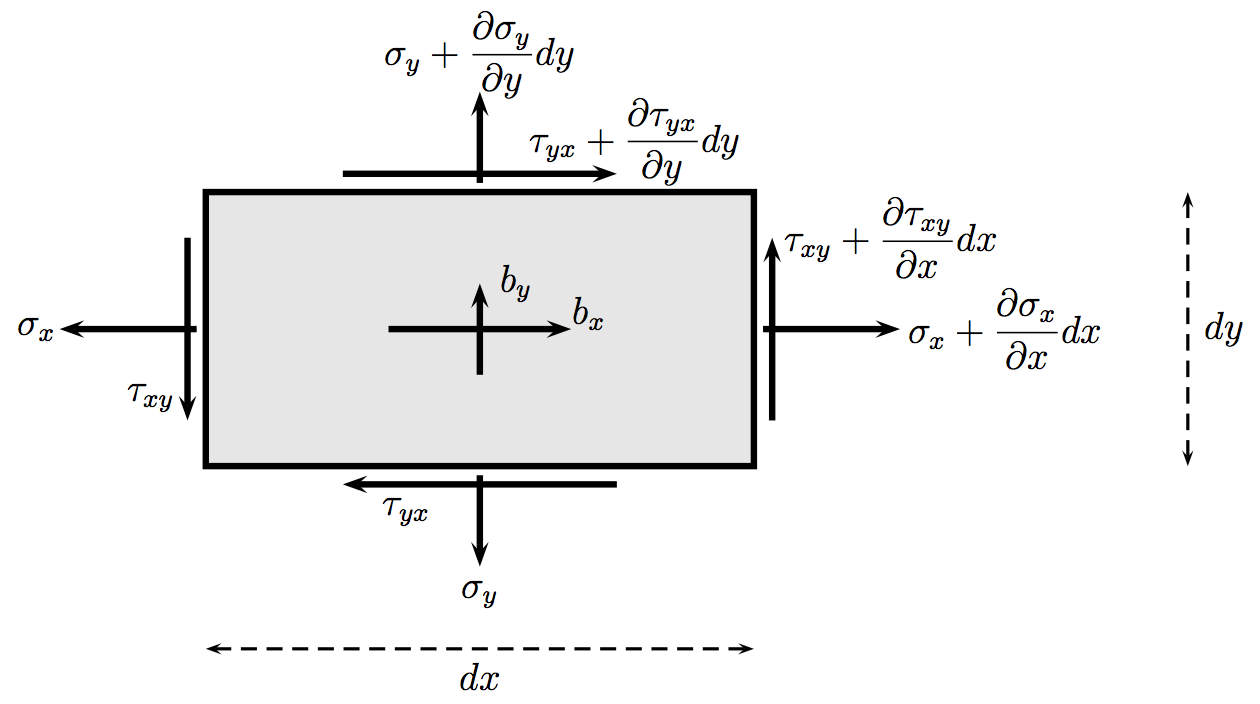
\includegraphics[scale=0.3]{ch3/4}
		\captionof{figure}{}
		\end{wrapfigure}		
		It is finally time to derive the equilibrium equations. Instead of compuing this for every point of a body, we will use an infinitesimal element $dx\, dy$ in 2D. By isolating this element, all forces (body and surface) acting on it should be balanced.  The balance on the x-axis gives:\\
		
		\begin{equation}
		\begin{aligned}
		&b_x\, dx\, dy + \left(\frac{D\sigma _x}{\D x}\, dx\right) dy + \left( \tau _{yx} + \frac{\D \tau _{yx}}{\D y}\, dy \right) dx- \sigma _x \, dy - \tau _{yx}\, dx=0\\
		\Leftrightarrow \qquad &b_x \,dx \, dy + \frac{\D \sigma_x}{\D x}dx\, dy + \frac{\D \tau _{yx}}{\D y} dx \, dy =0\\
		\Leftrightarrow \qquad &b_x + \frac{\D \sigma_x}{\D x} + \frac{\D \tau _{yx}}{\D y} =0
		\end{aligned}
		\end{equation}
		
		By using indicial notation, we can generalize this approach in 3D and get a set of three equilibrium equations in translation:
		
		\begin{equation}
		b_i + \tau _{ji,j} = 0
		\end{equation}
		
		where $i$ is a free or unrepeated index and $j$ a summed or dummy index. Here are some rules:
		
		\begin{itemize}
			\item[•] $\delta_{ij}$ is the \textbf{Kronecker delta} and $=1$ if $i=j$, $=0$ otherwise;
			
			\item[•] $\epsilon _{ijk}$ is the permutation symbol which is $=1$ if $ijk$ makes a positive permutation, $=-1$ if negative permutation and $=0$ otherwise (see syllabus if don't remember);
			
			\item[•] $u_iv_i$ is a scalar product of $\bm{u}$ and $\bm{v}$;
			\item[•] $\epsilon _{ijk} u_jv_k$ is a cross product;
			\item[•] $\epsilon _{ijk} \D _j u_k$ is the curl of $\bm{u}$ ($\nabla \times \bm{u}$);
			\item[•] Gauss theorem in indicial notation:
			\begin{equation}
			\int _V u_{i,i}\, dV = \oint u_i n_i \, dS.
			\end{equation}
\end{itemize}		 

			\ \\ Now we have also to verify the rotation equilibrium. If the reference point is the origin of the axes, we denote $x_i$ the current position, then the rotation equilibrium for an arbitrary volume $V' \in V$ delimited by $S'$ is:
			
			\begin{equation}
			\int _{V'} \epsilon _{ijk} x_j b_k\, dV' + \oint _{S'}\epsilon _{ijk} x_j t^{(n)}_k \, dS' = 0 
			\end{equation}
			where we applied the definition of the moment position $\times$ force. We know that $t^{(n)}_k = \tau _qk n_q$. By using this and the Gauss theorem we obtain:
			
			\begin{equation}
			\begin{aligned}
			&\int _V \epsilon _{ijk}\left[ x_j b_k + (x_j \tau _{qk},q)\right] dV' = \int _V \epsilon _{ijk}\left[ x_j b_k + x_j \tau _{qk,q} +x_{j,q} \tau _{qk} \right] dV'\\
			=\qquad &\int _V \epsilon _{ijk}\left[ x_j\underbrace{(b_k + \tau _{qk,q})}_{=0} +x_{j,q} \tau _{qk} \right] dV' = \int _V \epsilon _{ijk} x_{j,q} \tau _{qk} \, dV' = 0.
			\end{aligned}
			\end{equation}
			 Remark that $x_{j,q} = \delta _{jq}$, and since $V'\in V$ is completely arbitrary the integral must vanish:
			 
			 \begin{equation}
			 \epsilon _{ijk} \tau _{jk}= 0.
			 \end{equation}
			 
			 We can conclude that \textbf{in the absence of concentrated body moments, the stress tensor is symmetric.} We revise our equation to
			 
			 \begin{center}
			 \theor{
			 \begin{equation}
			 \tau _k^{(n)} = \tau _{kq} n_q \quad ; \quad b_i + \tau _{ij,j} = 0\quad ; \quad \tau _{ij} = \tau _{ji} 
			 \end{equation}
			 }
			 \end{center}
			 
		\subsection{Kinematics}
			\begin{wrapfigure}[9]{l}{7cm}
			\vspace{-5mm}	
			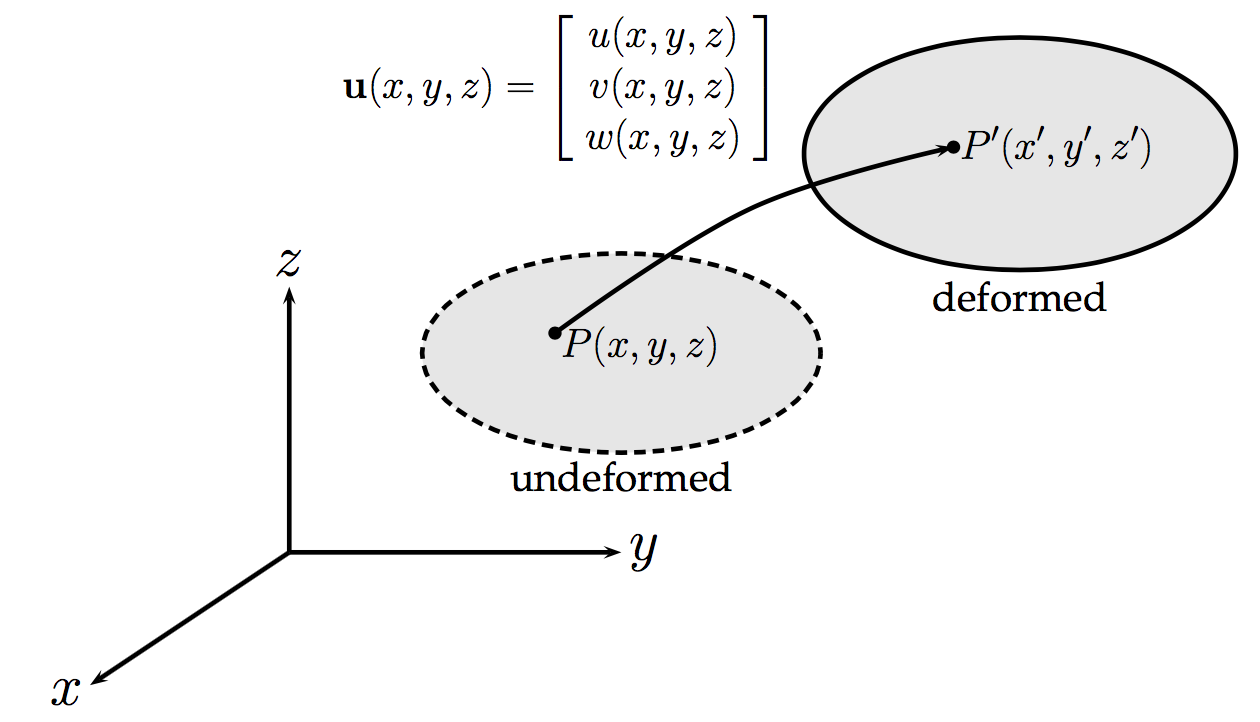
\includegraphics[scale=0.3]{ch3/5}
			\captionof{figure}{}
			\end{wrapfigure}		
			Continuum mechanics is also concerned by the way the volume is deformed through displacement and strains. Consider the volume V which is deformed in V' by applying a \textbf{displacement} on each point of V. In much applications the displacement can be assumed to be much smaller than the dimensions of the volume, leading to the \textbf{infinitesimal strain theory}, also called \textbf{small displacement-gradient theory}. \newpage 
			
			This simplifies our live because we assume the deformed volume to remain as the initial one and we can perform the integrals interchangeably on the initial or deformed configuration. This is valid for stiff materials like steel. Other flexible materials are the scope of non linear mechanics. The \textbf{linear strain tensor} is derived from the displacement field:
			
			\begin{equation}
			\epsilon _{ij}= \frac{1}{2} (u_{i,j + u_{j,i}})\qquad \bm{\bar{ \bar{\epsilon}}} = 
			\left[
			\begin{array}{ccc}
			\epsilon _x &\frac{\gamma _{xy}}{2} &\frac{\gamma _{xz}}{2} \\
			\frac{\gamma _{yx}}{2} & \epsilon _y & \frac{\gamma _{yz}}{2}\\
			\frac{\gamma _{zx}}{2} & \frac{\gamma _{zy}}{2} & \epsilon _z
			\end{array}						
			\right]
			\end{equation}
			
			where the $\epsilon _i$ are the axial strain and the $\gamma _{ij}$ are the shear strain. \textbf{Don't forget the importance of small displacements!}
			
	\section{Linear elasticity}
		\subsection{Material law}
			\begin{wrapfigure}[8]{l}{5.5cm}
			\vspace{-5mm}	
			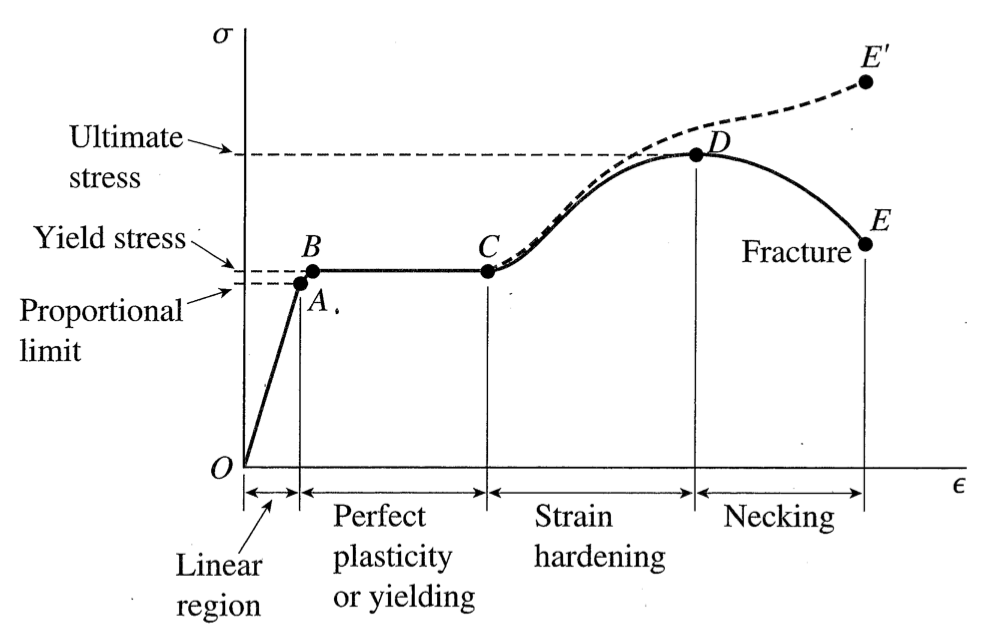
\includegraphics[scale=0.3]{ch3/6}
			\captionof{figure}{}
			\label{fig:3.6}
			\end{wrapfigure}		
			The understanding of the mechanical response requires a link between stresses and strains. This is done by the \textbf{material law}. It is find experimentally, using a tensile test machine that loads the material in tension at a constant speed until fracture. The \textbf{nominal axial stress} and the \textbf{average axial strain} are obtained respectively by dividing the force and the displacement by the initial surface and length of the sample:
			
			\begin{equation}
			\sigma = \frac{P}{A_0} \qquad \epsilon = \frac{\delta}{L_0.}	
			\end{equation}			 
			
			On \autoref{fig:3.6}, the O state corresponds to no strain no stress, then a straight line to A. The slope of OA is called the \textbf{modulus of elasticity} or the \textbf{Young's modulus}, noted E [$N/m^2$]. After A, the relation is no longer linear. In AB the strain increases more rapidly than the strain, until a plateau BC where large strains are obtain without increase of load, \textbf{perfect plasticity}. The constant stress at this stage is the \textbf{yield stress}. \\
			
			After this, the material \textbf{strain harden}, it resists to further deformation. The maximum stress is the \textbf{ultimate stress} on D. Then, the section A is shrunk and the bar is necking. The load decreases until the failure. By using the "true" cross-section area $A_{true}$, we can draw a true stress-strain curve CE'. We will focus on \textbf{linear elastic materials}. Elasticity points that $\sigma$ is a unique function of $\delta$ and that the material recovers initial state when unloaded. Linearity points to the proportionality. \\
			
			\begin{wrapfigure}[8]{r}{4cm}
			\vspace{-10mm}	
			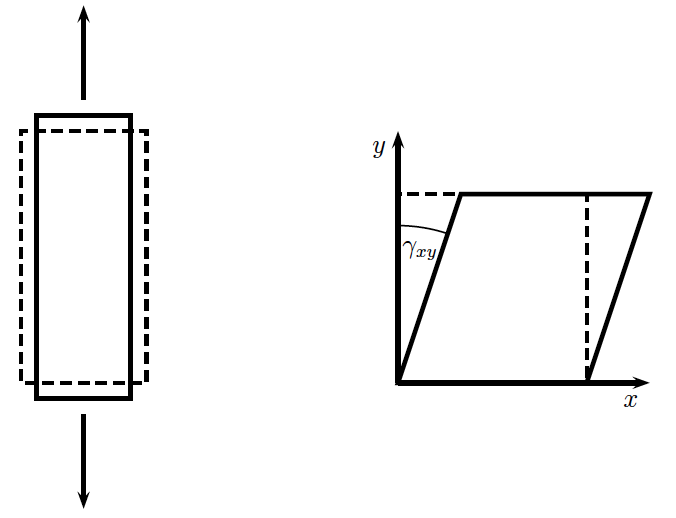
\includegraphics[scale=0.3]{ch3/7}
			\captionof{figure}{}
			\label{fig:3.7}
			\end{wrapfigure}		
			Additionally to the axial deformation, in prismatic bar is accompanied by a \textbf{lateral contraction} from the very beginning of the load. In the elastic domain, this is the \textbf{Poisson effect}: 
			
			\begin{equation}
			\epsilon _x = \frac{\sigma _x}{E} , \qquad \epsilon _y = \epsilon _z = - \frac{\nu \sigma _x}{E}
			\end{equation}
			
			where $0\leq\nu\leq 0.5$ is the Poisson coefficient. Let's remark that similarly to the Hooke's law, a shear version can be:
			
			\begin{equation}
			\tau = G \gamma \qquad G =\frac{E}{2 (1+\nu )}
			\end{equation}
			
			where the shear strain $\gamma _{xy}$ can be interpreted as the angular deformation in xy. In 3D, as $\tau _{ij}$ and $\epsilon _{ij}$ are second order tensors, we need a fourth-order tensor $C_{ijkl}$ such that $\tau _{ij} = C_{ijkl} \epsilon _{kl}$. This is simplified for \textbf{isentropic elastic materials}:
			
			\begin{equation}
			\tau _{ij} = \lambda \epsilon _{kk} + 2\mu \epsilon _{ij}
			\end{equation}
			
			where $\lambda, \mu$ are the \textbf{Lamé constants}, defined as:
			
			\begin{equation}
			\lambda = \frac{\nu E}{(1+\nu) (1-2\nu) }, \qquad \mu = \frac{E}{2(1+\nu)} = G.
			\end{equation}
			
			Finally, if we replace we get 
			
			\begin{center}
			\theor{
			\textbf{Stress-strain relationship in isotreopic elasticity}
			\begin{equation}
			\epsilon _{ij} = \frac{1}{E }[(1+\nu) \tau _{ij} - \nu \delta _{ij} \tau _{kk}].
			\end{equation}						
			}
			\end{center}
			
			In general material have also a non-linear behavior, but as in engineering we design the material to remain below the linear limit, we can make the approx. 
			
\subsection{Strain energy}
	\begin{wrapfigure}[8]{r}{4.5cm}
	\vspace{-5mm}	
	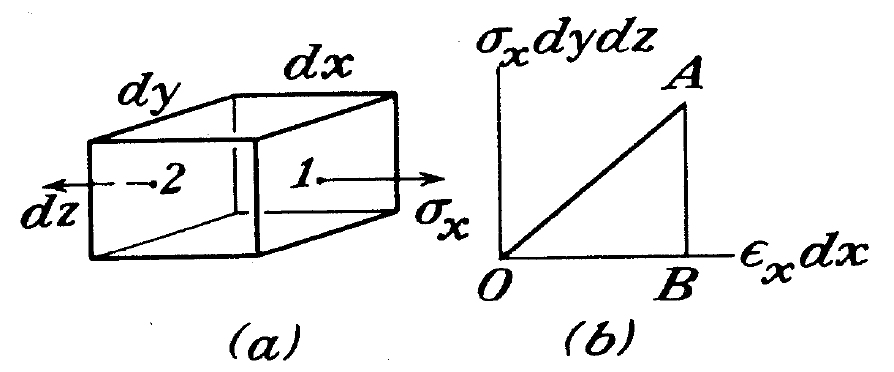
\includegraphics[scale=0.3]{ch3/8}
	\captionof{figure}{}
	\label{fig:3.8}
	\end{wrapfigure}	
	When a load is applied, the external work of the force is converted into strain energy. Indeed, the application of $\sigma _x$ induces an extension $\epsilon _x dx$ , physically the energy for a volume is:
	
	\begin{equation}
	dW = \frac{1}{2} \sigma _x \epsilon _x \, dx\, dy\, dz.
	\end{equation}
	
	In the general case, the conservation of energy for linear elastic materials, the work cannot depend on the order of magnitude of the load. In other word, we have to multiply stress and strain tensors component by component:
	\begin{equation}
	\begin{aligned}
	dW &= W_V \, dx\, dy\, dz = \frac{1}{2} \tau _{ij} \epsilon _{ij} \, dx\, dy\, dz.\\
	&= \frac{1}{2} (\sigma _x \epsilon _x +\sigma _y \epsilon _y+\sigma _z \epsilon _z + \tau _{xy}\epsilon _{xy}+ \tau _{xz}\epsilon _{xz}+ \tau _{yz}\epsilon _{yz} + \tau _{yx}\epsilon _{yx}+ \tau _{zx}\epsilon _{zx}+ \tau _{zy}\epsilon _{zy}) \, dx\, dy\, dz\\
	&= \frac{1}{2} (\sigma _x \epsilon _x +\sigma _y \epsilon _y+\sigma _z \epsilon _z + \tau _{xy}\gamma _{xy}+ \tau _{xz}\gamma _{xz}+ \tau _{yz}\gamma _{yz}) \, dx\, dy\, dz
	\end{aligned}
	\end{equation}
	
	where $W_V$ is the \textbf{strain energy density}:
	$W_V = \int _{\epsilon _{ij}} \tau _{ij} \, d\epsilon _{ij}.$
	
	We see the utility of defining $\epsilon _{xy} = \frac{1}{2} \gamma _{xy}$ in the equation. Using the Hooke's law:
	
	\begin{equation}
	\begin{aligned}
	W_V &= \frac{1}{2E}(\sigma _x ^2 + \sigma _y ^2 +\sigma _z ^2) - \frac{\nu }{E} ( \sigma _x\sigma _y + \sigma _x\sigma _z + \sigma _y \sigma _z) + \frac{1}{2G} (\tau _{xy}^2+\tau _{xz}^2+\tau _{yz}^2)\\
	&= \frac{1}{2}\lambda (\epsilon _x ^2+\epsilon _y ^2+\epsilon _z ^2) + G(\epsilon _x ^2+\epsilon _y ^2+\epsilon _z ^2) + \frac{1}{2} G (\gamma _{xy}^2 +\gamma _{xz}^2 + \gamma _{yz}^2).
	\end{aligned}
	\end{equation}
	
	We see that $W_V$ is always \textbf{positive}. Let's define the dual $W_V^* = \int _{\tau _{ij}} \epsilon _{ij} \, d\tau _{ij}$, such that:
	
	\begin{equation}
	W_V + W_V^* = \tau _{ij} \epsilon _{ij}.
	\end{equation}
	
	The strain energy W and the complementary are obtained by $\int _V W_V\, dV$, with $W_V = W_V^* = \frac{1}{2}\tau _{ij}\epsilon _{ij}$.